\documentclass[12pt]{article}
\usepackage[english]{babel}
\title{StatCrunch Competition\\ Twitch Dataset}
\author{Matthew Carson\\ University of California, Los Angeles}
\date{\today}
\usepackage{url}
\usepackage{hyperref}
\usepackage{amsmath}
\usepackage{graphicx}
\usepackage{caption} % for customizing captions
\usepackage[margin=1in]{geometry} % for setting margins
\usepackage{setspace} % for adjusting line spacing
% Line spacing
\setstretch{1.25}
\usepackage[autostyle, english = american]{csquotes}
\MakeOuterQuote{"}

% Define indentation length
\newlength{\myindent}
\setlength{\myindent}{3em}

% Paragraph indentation
\setlength{\parindent}{\myindent}

%%%%%%%%%%%%%%%%%%%%%%%%%%%%%
% Begin Document
% Title Page
%%%%%%%%%%%%%%%%%%%%%%%%%%%%%
\begin{document}
\begin{titlepage}
\maketitle
\thispagestyle{empty} % Removes page number from the cover page
\end{titlepage}
% Set page numbering to roman for preliminary pages
\pagenumbering{roman}
%%%%%%%%%%%%%%%%%%%%%%%%%%%%%
% Table of Contents
%%%%%%%%%%%%%%%%%%%%%%%%%%%%%
\tableofcontents
%\newpage

%%%%%%%%%%%%%%%%%%%%%%%%%%%%%
% List of Figures
%%%%%%%%%%%%%%%%%%%%%%%%%%%%%
\listoffigures
%\newpage

%%%%%%%%%%%%%%%%%%%%%%%%%%%%%
% List of Tables
%%%%%%%%%%%%%%%%%%%%%%%%%%%%%
\listoftables
\newpage
%%%%%%%%%%%%%%%%%%%%%%%%%%%%%
% Begin body of report
%%%%%%%%%%%%%%%%%%%%%%%%%%%%%
% Set page numbering to arabic for main content
\pagenumbering{arabic}

\section{Summary Statistics}\

Since these data were not randomly sampled, it would be inappropriate to conduct inference (i.e., construct confidence intervals or conduct hypothesis tests). Because of this, it is not possible to estimate population parameters; that is, make claims or generalizations about the broader population of Twitch users. However, since these data represent the top 900 Twitch users, statistics can be calculated and relationships can be discovered about that population.

Initial calculations were made before presenting the summary statistics. Since values for \texttt{`Watch time (mins)'} were typically very large, requiring scientific notation to express, values were rescaled to \texttt{`Mean weekly watch hours’} by dividing \texttt{`Watch time (mins)'} by the product of 60 times 52 (number of weeks in a year) to make the numbers more manageable:

\begin{equation}
Mean\ weekly\ watch\ hours = \dfrac{Watch\ time\ (mins)}{60 \ast 52}
\end{equation}
\newline
Additional statistics were calculated as well:

\begin{itemize}
	\item \texttt{`Followers Prev Yr’} = \texttt{`Followers’} - \texttt{`Followers gained’}.
	\item \texttt{`Followers gained percent’} = \texttt{`Followers gained’} / \texttt{`Followers Prev Yr’}.
\end{itemize}

Because all distributions are heavily right skewed (skewness $\geq$ 2.6), medians, represented with Greek letter eta ($\eta$), are reported instead of means (all values are from Table \ref{fig:summary_stats}). The majority of the top nine hundred accounts stream content at least 30 hours per week ($\eta \approx$ 34.23) and are watched more than 90 thousand hours per week $(\eta \approx$ 91,422). Most accounts gained a substantial number of followers from the previous year ($\eta \approx$ 66,003), which represents a median increase of approximately 16 percent. Because of the heavy skewness of the distributions, easy-to-interpret visualizations were difficult to make (Figure \ref{fig:histogram_matrix}).

%%%%%%%%%%%%%%%%%%%%%%%%%%%%%
% Table: Summary Statistics
%%%%%%%%%%%%%%%%%%%%%%%%%%%%%
\begin{table}[ht]
  \centering
  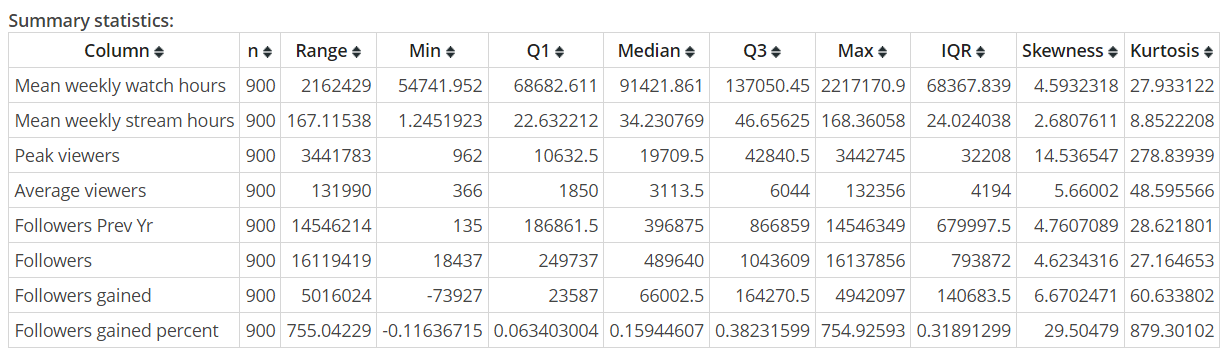
\includegraphics[width=\linewidth]{../StatCrunch_Results/table}
  \captionsetup{justification=centering, singlelinecheck=false, margin=2cm}
  \caption[Summary Statistics]{Summary Statistics.}
  \label{fig:summary_stats}
\end{table}

\section{Correlation}

To assess the relationships between numeric variables, Spearman’s correlation coefficients were calculated. Because of the non-linearity of the relationships (Figure \ref{fig:stream_scatter_matrix}), typical Pearson’s R correlation coefficients would be inappropriate. Spearman’s correlation coefficients are preferred for assessing the strength of non-linear relationships.

The relationships between numeric variables are surprising, especially the absence of some correlations where one would think they they would exist (Figure \ref{fig:spearman_correlogram}). \texttt{`Stream time’} has a moderately strong negative Spearman correlation ($\rho$) with \texttt{`Average viewers’} ($\rho = -0.63$), which is counterintuitive given that one might expect more frequent streaming to result in more viewers, but that is not the case. In terms of change over time, accounts that streamed for more hours   With respect to surprising absences of relationships, \texttt{`Stream time’} has practically no relationship with \texttt{`Watch time’} ($\rho = 0.07$; Figure \ref{fig:spearman_correlogram}). Together, these findings suggest that a strategy of merely increasing one’s streaming time does not “pay off” in terms of the number of followers or viewers.

%%%%%%%%%%%%%%
% Figure: Spearman Correlogram
%%%%%%%%%%%%%%
\begin{figure}[hb]
  \centering
  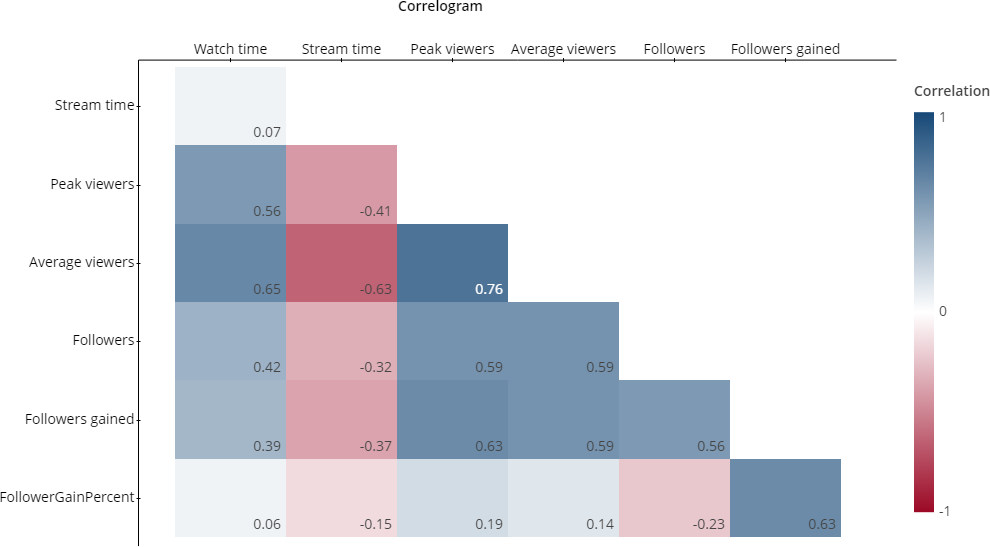
\includegraphics[width=\linewidth]{../StatCrunch_Results/spearman_correlogram}
  \captionsetup{justification=centering, singlelinecheck=false, margin=2cm}
  \caption[Spearman Correlogram]{Spearman Correlogram}
  \label{fig:spearman_correlogram}
\end{figure}

%%%%%%%%%%%%%
% Figure: Histogram Matrix
%%%%%%%%%%%%%
\begin{figure}[h]
  \centering
  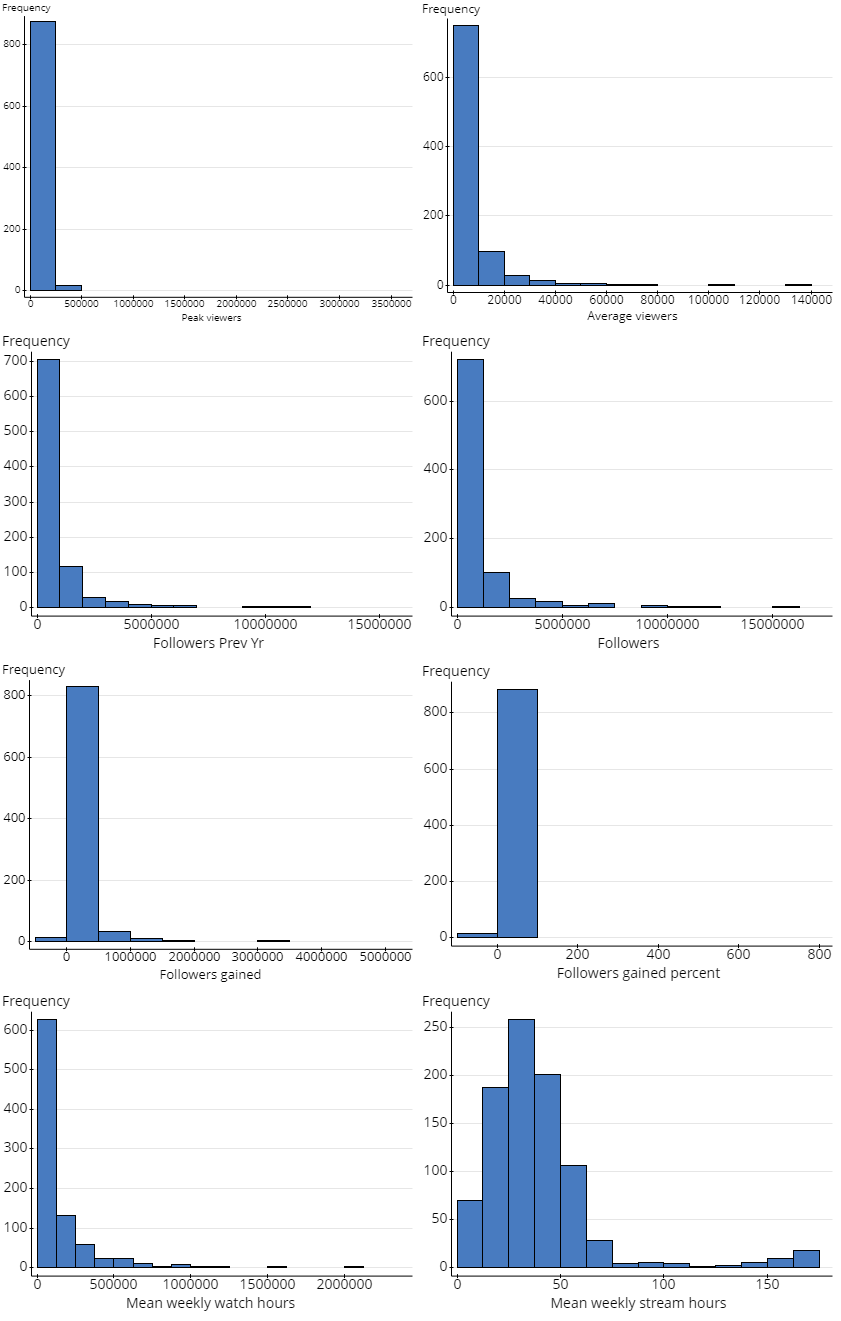
\includegraphics[width=0.8\linewidth]{../StatCrunch_Results/Histogram_Matrix.png}
  \captionsetup{justification=centering, singlelinecheck=false, margin=2cm}
  \caption[Histogram Matrix]{All distributions are heavily skewed and non-normal.}
  \label{fig:histogram_matrix}
\end{figure}

%%%%%%%%%%%%%%%%%%%
% Figure: Stream Hours Scatter Plot Matrix
%%%%%%%%%%%%%%%%%%%
\begin{figure}
  \centering
  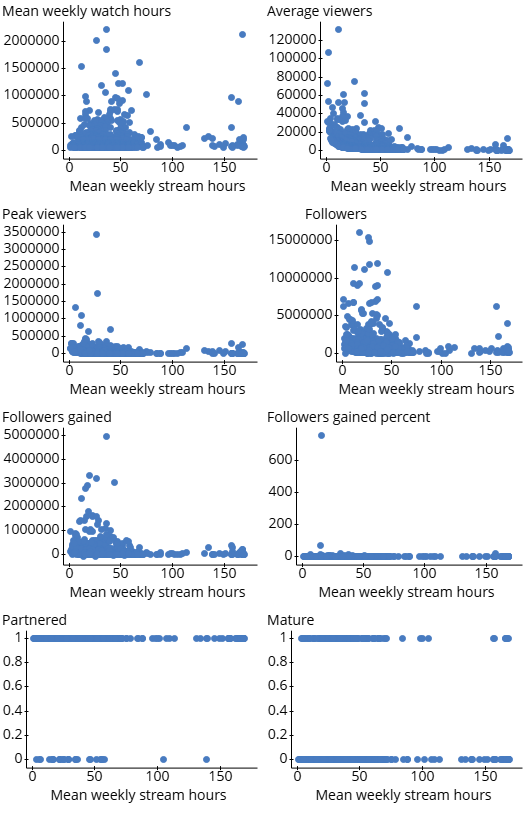
\includegraphics[width=0.8\linewidth]{../StatCrunch_Results/stream_scatter_plot_matrix.png}
  \captionsetup{justification=centering, singlelinecheck=false, margin=2cm}
  \caption[Stream Hours Scatter Plot Matrix]{Relationships between \texttt{`Mean weekly stream hours'} and other variables.}
  \label{fig:stream_scatter_matrix}
\end{figure}

%%%%%%%%%%%%%%%%%%%%%%%%%%%%%%%%%%%%%%%%%%%%
% Figure: Watch Hours Scatter Plot Matrix
%%%%%%%%%%%%%%%%%%%%%%%%%%%%%%%%%%%%%%%%%%%%
\begin{figure}
  \centering
  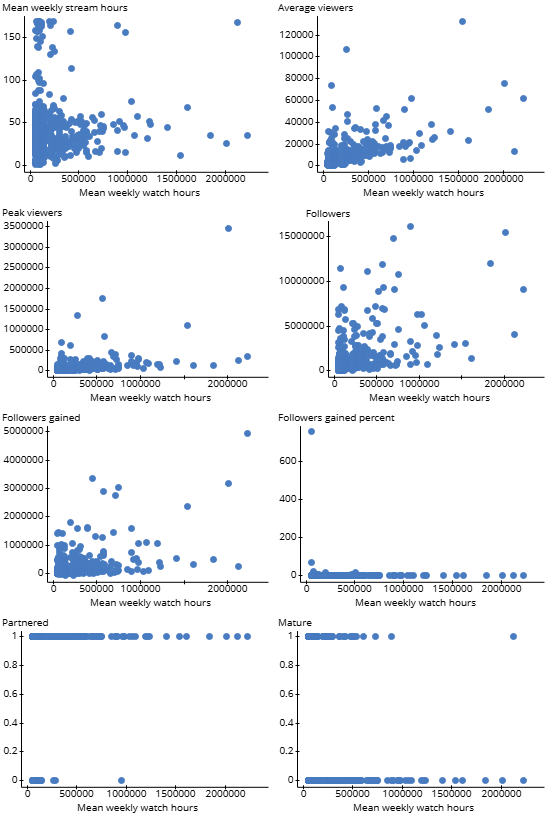
\includegraphics[width=0.8\linewidth]{../StatCrunch_Results/watch_scatter_plot_matrix.png}
  \captionsetup{justification=centering, singlelinecheck=false, margin=2cm}
  \caption[Watch Hours Scatter Plot Matrix]{Relationships between \texttt{`Mean weekly watch hours'} and other variables.}
  \label{fig:watch_scatter_matrix}
\end{figure}

%%%%%%%%%%%%%%%%%%%%%%%%
% Figure: Followers Gained Scatter Plot Matrix
%%%%%%%%%%%%%%%%%%%%%%%%
\begin{figure}
  \centering
  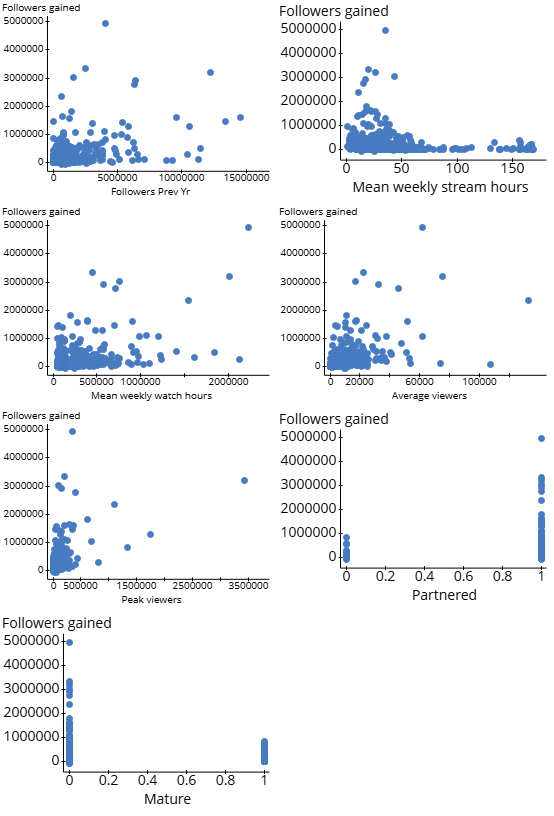
\includegraphics[width=0.8\linewidth]{../StatCrunch_Results/follow_gain_scatter_matrix}
  \captionsetup{justification=centering, singlelinecheck=false, margin=2cm}
  \caption[Followers Gained Scatter Plot Matrix]{Relationships between \texttt{`Followers gained'} and other variables.}
  \label{fig:follow_gain_scatter_matrix}
\end{figure}


% ceil(Rank(Mean weekly stream hours) / 90)

\end{document}